\chapter{绪论}
\label{cha:chap1}
\section{研究背景和研究意义}
\label{sec:1.1}
基于
\subsection{研究背景}
\label{sec:1.1.1}
基于
\subsection{研究意义}
\label{sec:1.1.2}
基于
\section{国内外研究现状}
\label{sec:1.2}
基于
\subsection{SLAM的研究现状}
\label{sec:1.2.1}
即时定位与地图构建是让机器人在未知环境中持续地构建环境地图,并同时在地图中给自己定位。最早的SLAM技术还不是使用视觉的方法,
而是使用声波传感器或者激光以及惯性测量单元实现环境建模和自身定位。直到21世纪,Stephen Se等人首次使用图像的特征点实现视觉
SLAM\cite{se2002mobile},之后由Davison使用EKF框架实现了最早的单目实时SLAM系统\cite{davison2003real},奠定了单目系统
的基础;Davison在2007年成功实现基于单相机的纯视觉SLAM系统,算法的关键是在线建立2D点到3D点的映射关系,并且使用实时运动模
型估计相机的位置\cite{davison2007monoslam};Mur-Artal使用ORB特征点作为地图构建特征点,大幅度降低了点云的数量,并且使用
回环检测的方法使定位与建图的精度都大幅提升\cite{mur2015orb};随着硬件计算能力和数据储存的提升,提取目标深度信息的技术得
到了很大的发展,戚传江等人使用2D slam的解决方案,采用多传感器数据融合的方法,完成多自由度位姿检测,拓展了SLAM的应用场
景;Whelan的实验通过使用体积融合的方法实现了实时大范围的稠密RGB-D的SLAM系统\cite{whelan2015real},通过这个研究,使用
SLAM系统作三维环境构建以及实时相机定位成为可能。

应用到目标跟踪领域,单纯点云集还是无法满足要求,因此需要将点云数据语义化,Reiger使用关系树的方法实现物体的语义识别
\cite{sarkar2012slam},这项技术对于目标跟踪是很重要的;之后Sarkar在Reiger的研究基础上结合FastSLAM的方法,使得识别速度更
快,鲁棒性更强;Zhang, G等人使用基于线条的SLAM算法\cite{zhang2015building}提高物体识别的准确率,该方法能够对物体的边沿与
轮廓进行稳定的识别。

\subsection{三维重建的研究现状}
\label{sec:1.2.2}
照相机/摄像机是将一个三维场景或物体投影到二维平面上,但是在降维的过程不可避免地会损失存在信息,而利用三维重建技术,就是从获
取到的二维图像中复原原始三维场景或物体,三维重建的结果如图~\ref{fig:3d_constr}所示。

\begin{figure}[H] % use float package if you want it here
    \centering
    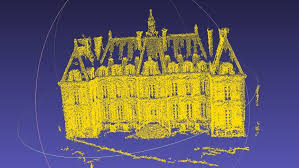
\includegraphics[height=8cm]{3d_constr.png}
    \caption{三维重建结果示意图}
    \label{fig:3d_constr}
  \end{figure}
  
CMU大学的Tomasi和Kanade\cite{tomasi1992shape}等人首先开发出了基于图片的三维重建系统,并利用仿射分解法对摄像机进行了标定,
得到摄像机运动参数,然后重构出物体的空间模型。随后,INRIAB Bougnoux等人\cite{bougnoux1997totalcalib,debevec1998image}
利用未标定的SfM和摄像机自标定等算法,开发了一个提升型三维重建模型。Berkeley大学的Debevoc\cite{beardsley19963d}等人完成了
著名的建筑物重构系统Façade,该系统要求首先得到建筑物的粗略几何模型和摄像机运动参数。Shum等人开发的人机交互式重构系统,利用
物体的一组全景图,即从各个角度得到物体的n张图片,然后对这些图像进行处理,重构出其三维实体,或者将场景表示成一系列按深度划分
的分层的集合。Faugeras等采用摄像机的自标定方法,利用分层重构等经典的方法,从图像序列中重构出建筑物的形貌。Katholieke大学
的Pollefeys等提出物体表面自动生成系统,该系统是在内参数可以改变的情况下,对摄像机采取了自标定的技术,该系统只要求用摄像机
绕物体周围一周,拍到一系列的图像,就可以自动实现自标定和分层重构。

\subsection{基于视觉体积测算的研究现状}
\label{sec:1.2.3}
基于
\subsection{语义结构化地图的研究现状}
\label{sec:1.2.4}
基于
\section{待解决问题}
\label{sec:1.3}
基于
\section{主要研究内容和技术路线}
\label{sec:1.4}
基于
